\documentclass[border=3pt]{standalone}
% Preâmbulo compartilhado pelos diagramas TikZ da aula 8 de IHC (Design de IHC)
\usepackage[T1]{fontenc}
\usepackage[utf8]{inputenc}
\usepackage{lmodern}
\usepackage{amsmath}
\usepackage{xcolor}
\usepackage{tikz}
\usetikzlibrary{arrows.meta,angles,quotes,decorations.pathmorphing,decorations.pathreplacing,calc,
                positioning,shapes.geometric,shapes.misc,backgrounds,fit,
                math}

% Paleta (mesma dos SVGs originais)
% Paleta da disciplina de IHC: acento roxo (#755099), da capa do livro.
% (o nome "dblue" é mantido para não alterar todos os diagramas)
\definecolor{dblue}{HTML}{755099}
\definecolor{dorange}{HTML}{B3541E}
\definecolor{dgreen}{HTML}{4A7C59}
\definecolor{dred}{HTML}{9C4B4B}
\definecolor{dcream}{HTML}{F4F1EA}
\definecolor{dshade}{HTML}{DDD7C9}

% Função gaussiana (não normalizada por padrão de escala visual)
\pgfmathdeclarefunction{gauss}{3}{%
  \pgfmathparse{1/(#3*sqrt(2*pi))*exp(-((#1-#2)^2)/(2*#3^2))}%
}

% Estilos comuns (prefixo d... para não colidir com chaves internas do pgf)
\tikzset{
  >={Stealth[length=2mm]},
  dguide/.style={gray!55, dashed, line width=0.4pt},
  daxis/.style={gray!60, line width=0.7pt, ->},
  dbody/.style={fill=black!3, draw=black!80, line width=1pt},
  dacc/.style={draw=dblue, line width=1pt},
  dlbl/.style={black!55, font=\small},
  dsub/.style={black!45, font=\footnotesize},
  dstate/.style={circle, draw=black!80, fill=dcream, line width=1pt,
                 minimum size=17mm, font=\large, inner sep=1pt},
  dobs/.style={circle, draw=black!80, fill=dshade, line width=1pt,
               minimum size=14mm, font=\large, inner sep=1pt},
  dbox/.style={rounded corners=2pt, draw=black!80, fill=dcream, line width=1pt,
               align=center, inner sep=6pt},
  dop/.style={circle, draw=black!80, fill=white, line width=1pt,
              minimum size=6mm, inner sep=0pt, font=\small},
  dtrans/.style={->, dblue, line width=1pt},
  dmeas/.style={->, dorange, line width=1pt},
  dcurve/.style={line width=1pt, dblue},
  dcurveb/.style={line width=1.4pt, dorange},
}

\begin{document}
\hyphenpenalty=10000 \exhyphenpenalty=10000 \tolerance=9999 \emergencystretch=3em
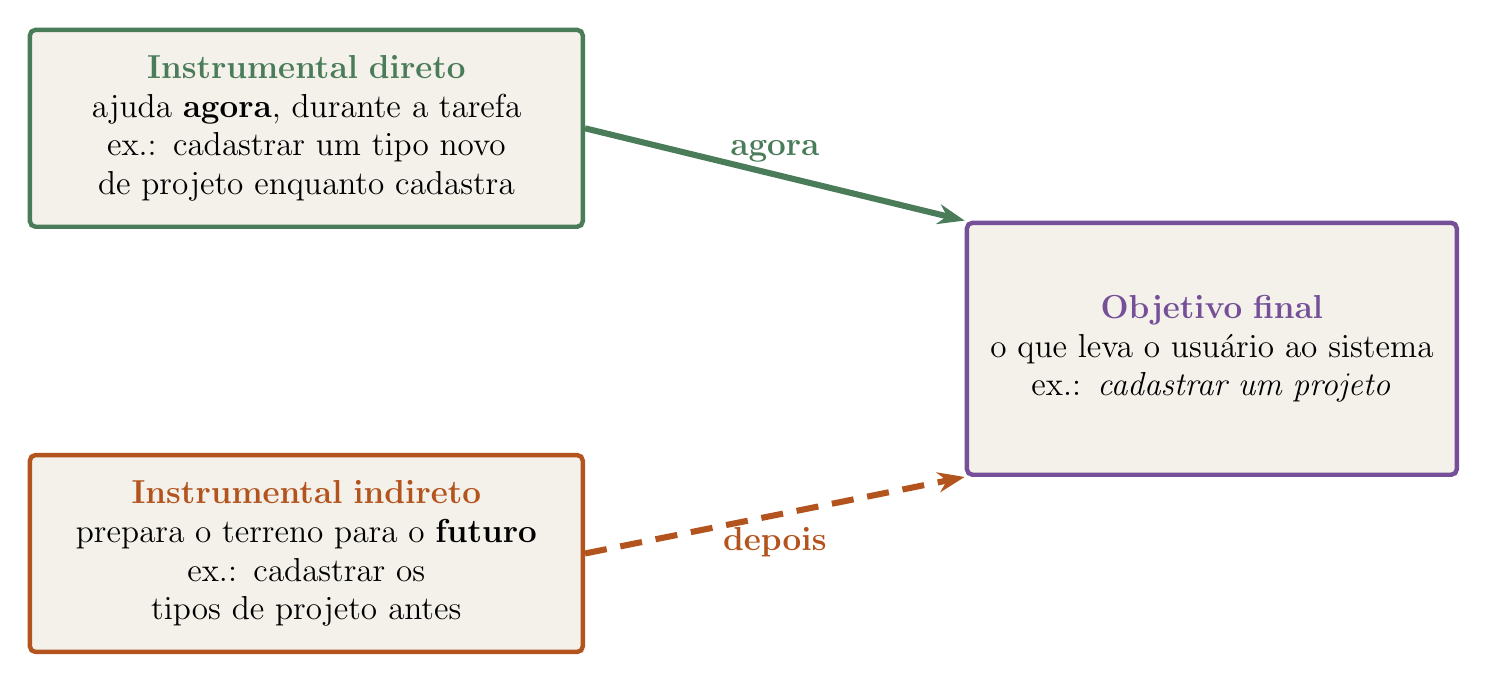
\begin{tikzpicture}[x=1cm,y=1cm]
\tikzset{c/.style={dbox, text width=6.6cm, minimum height=2.5cm, font=\large, line width=1.6pt}}
\node[c, draw=dblue, text width=5.8cm, minimum height=3.2cm] (f) at (15.5,4.4) {\textbf{\textcolor{dblue}{Objetivo final}}\\ o que leva o usuário ao sistema\\ ex.: \emph{cadastrar um projeto}};
\node[c, draw=dgreen] (d) at (4.0,7.2) {\textbf{\textcolor{dgreen}{Instrumental direto}}\\ ajuda \textbf{agora}, durante a tarefa\\ ex.: cadastrar um tipo novo de projeto enquanto cadastra};
\node[c, draw=dorange] (i) at (4.0,1.8) {\textbf{\textcolor{dorange}{Instrumental indireto}}\\ prepara o terreno para o \textbf{futuro}\\ ex.: cadastrar os tipos de projeto antes};
\draw[dgreen, line width=2.2pt, -{Stealth[length=3.4mm]}] (d.east) -- node[above, font=\large\bfseries, dgreen] {agora} (f.north west);
\draw[dorange, line width=2.2pt, dash pattern=on 8pt off 5pt, -{Stealth[length=3.4mm]}] (i.east) -- node[below, font=\large\bfseries, dorange] {depois} (f.south west);
\end{tikzpicture}
\end{document}
